\chapter{Using Explicit Locks} 
\label{chap:locks}

So far in this book, we have concentrated on message-passing concurrency,
together with barrier synchronisations to synchronise threads.  In the next
few chapters, we will look at other concurrency primitives.  These typically
operate at a lower level of abstraction.  They are often built in to the
hardware, the operating system, or the programming language implementation.
This tends to make them more efficient.  However, they tend to be harder to
use, and less intuitive, than message passing, which is why we started this
book with the latter.

In this chapter we will see how to use explicit locks.  An SCL lock can be
created as follows:
%
\begin{scala}
  val lock = new Lock
\end{scala}

A lock has two principle operations:
%
\begin{itemize}
\item |acquire()|: wait until no other thread holds the lock, and then acquire
  it;

\item |release()|: release the lock.
\end{itemize}
%
At most one thread can hold the lock at a time.  Hence this gives us a way to
enforce mutual exclusion, for example, to avoid races.

We will see other uses of locks in the next chapter. 
%
Most other programming languages provide an implementation of locks with a
similar interface.

Figure~\ref{fig:counter-lock0} gives a simple example, based on the counter
example from Chapter~\ref{chap:intro}.  A lock is used to protect the counter
variable~|c|.  Each operation accesses~|c| only when it is holding the lock.
This means that it accesses~|c| under mutual exclusion, so two different
operations cannot interfere.

%%%%%

\begin{figure}
\begin{scala}
class Counter0{
  /** The value of the counter. */
  private var c = 0

  /** Lock used to protect £c£. */
  private val lock = new Lock

  /** Increment the counter. */
  def inc() = { lock.acquire(); c += 1; lock.release() }

  /** Decrement the counter. */
  def dec() = { lock.acquire(); c -= 1; lock.release() }

  /** Get the value of the counter. */
  def get: Int = { lock.acquire(); val result = c; lock.release(); result }
}
\end{scala}
\caption{A simple implementation of a counter, using a lock.}
\label{fig:counter-lock0}
\end{figure}

%%%%%

Note that the |get| operation copies the value of~|c| into a local
variable~|result| before releasing the lock and returning~|result|.  There are
a number of variants that do \emph{not} work, including the following.
\begin{itemize}
\item \SCALA{def get1: Int = \{ lock.acquire(); c; lock.release() \}}.  This
  does not work, because it doesn't return~|c|.  It returns the value of the
  final command in the sequence, namely |lock.release()|; this has type
  |Unit|, so in fact this definition doesn't typecheck.

\item \SCALA{def get2: Int = \{ lock.acquire(); return c; lock.release() \}}.
  This does not work, because it returns as soon as it reaches the |return|
  statement, so it doesn't release the lock!  No subsequent operation will be
  able to proceed.
\end{itemize}

\begin{instruction}
Make sure you understand the code in Figure~\ref{fig:counter-lock0}.
\end{instruction}

%%%%%

The |Lock| class also contains the following helper function, which performs
the computation~|comp| under mutual exclusion.
\begin{scala}
  /** Execute £comp£ under mutual exclusion for this lock. */
  def mutex[A](comp: => A): A = {
    acquire(); try{ comp } finally{ release() }
  } 
\end{scala}
%
(This is defined within the |Lock| class, to here |acquire| and |release| are
operations on the relevant lock object.)

The type ``\SCALA{=> A}'' means that the parameter |comp| is passed \emph{by
  name}.  Most parameters are passed in Scala are passed by value, which means
that they are evaluated \emph{before} the body of the function is executed.
That isn't what we want here, because it would mean that |comp| would be
evaluated before the lock is acquired, negating the intention!  Instead, the
computation |comp| is performed at the point it appears in the definition of
|mutex|, i.e.~after the lock is acquired.

The |finally| clause ensures that the lock is released after |comp| is
complete.  In particular, if |comp| returns a value, that value is calculated
and stored \emph{before} the lock is released: this avoids the necessity to
use a temporary variable discussed earlier.

Figure~\ref{fig:counter-lock} illustrates the use of the |mutex| function.
Every operation is simply wrapped inside an application of |mutex| on the
lock.  This makes it very each to provide mutual exclusion.  

%%%%%

\begin{figure}
\begin{scala}
class Counter extends CounterT{
  /** The value of the counter. */
  private var c = 0

  /** Lock used to protect c. */
  private val lock = new Lock

  /** Increment the counter. */
  def inc() = lock.mutex{ c += 1 }

  /** Decrement the counter. */
  def dec() = lock.mutex{ c -= 1 }

  /** Get the value of the counter. */
  def get: Int = lock.mutex{ c}
}
\end{scala}
\caption{A simple implementation of a counter, using a lock and {\scalashape
    mutex} blocks.}
\label{fig:counter-lock}
\end{figure}


Using |mutex| also means that if some code has several different branches, we
don't need to release the lock explicitly at the end of \emph{every} branch:
with explicit releasing, it is easy to miss a branch in such cases. 

%%%%%%%%%%%%%%%%%%%%%%%%%%%%%%%%%%%%%%%%%%%%%%%%%%%%%%%

%\subsection{Re-entry}

Consider an object that contains the following code
%
\begin{scala}
  private val lock = new Lock
  def f(x: Int) = lock.mutex{ ...; g(y); ... }
  def g(y: Int) = lock.mutex{ ... }
\end{scala}
%
Here the function~|f| calls the function~|g|, and both functions use a |mutex|
block.  That means that if a thread in~|f| gets to the call of~|g|, it already
holds the lock, but has to obtain it again.

The implementation of a |Lock| allows this: if a thread holds the lock, it can
acquire it again.  We say that the lock is \emph{re-entrant}.  Internally, the
implementation records how many times the thread holds the lock: it needs to
release the lock a corresponding number of times before another thread can
acquire it.  In the above example, if a thread in~|f| enters~|g|, it holds the
lock twice; when |g| returns, it holds the lock once; only when |f| returns
can another thread obtain the lock. 

%%%%%%%%%%  \heading{Java Memory Model}

Recall the discussion of memory caches from Chapter~\ref{chap:intro}: when a
thread reads a shared variable, it may read the value from its cache, and so
obtain an out-of-date version; when a thread writes to a shared variable,
initially the write happens only in the thread's cache, so the new value might
not be available to other threads.

Correct use of a |Lock| avoids these problems.  When a thread releases a
|Lock|, it \emph{publishes} the values in the cache, making them available to
other threads.  When a thread aquires a |Lock|, it \emph{subscribes} to all
variables published by other threads on the same |Lock|.  This means that if
all accesses to a variable are protected by a particular |Lock|, as in
Figure~\ref{fig:counter-lock}, then any read of the variable is guaranteed to
see the most-recent value written by another operation.  Further, compiler
optimisations must respect this semantics.  This means that if you are using
|Lock|s correctly to protect against data races, you do not need to worry
about the memory consistency.

%%%%%%%%%%%%%%%%%%%%%%%%%%%%%%%%%%%%%%%%%%%%%%%%%%%%%%%%%%%%

\section{Implementing Concurrent Objects with Locks}

A number of concurrent objects can be implemented using locks.  Remember, the
idea here is that a concurrent object should provide thread-safe operations:
executions of different executions should not interfere.  This can be achieved
by each operation execution locking the object, so as to provide mutual
exclusion.  This strategy is appropriate for \emph{total} operations, where
the operation can return a result in an arbitrary state.  However, it is no
appropriate for partial operations or synchronisation objects, where a thread
may have to wait: this will require an additional mechanism, which we will see
in the next chapter.

Figure~\ref{fig:LockTotalQueue} gives an implementation of a total queue (see
Section~\ref{sec:total-queue}), implemented using a lock.  Each of the main
operation simply performs the operation on the encapsulated |Queue|, while
achieving mutual exclusion using a |Lock|.  (We include the |shutdown|
operation simply to match the |TotalQueue| trait, but it is a no-op in this
case.) 

%%%%%

\begin{figure}
\begin{scala}
class LockTotalQueue[T] extends TotalQueue[T]{
  /** The current state of the queue. */
  private val queue = new Queue[T]

  /** A £Lock£ to protect queue. */
  private val lock = new Lock

  /** Enqueue £x£. */
  def enqueue(x: T) = lock.mutex{ queue.enqueue(x) }

  /** Try to dequeue.  Return £None£ if the queue is empty. */
  def dequeue(): Option[T] = lock.mutex{ 
    if(queue.isEmpty) None else Some(queue.dequeue()) 
  }

  /** Shutdown the queue. */
  def shutdown() = {} // Nothing to do.
}
\end{scala}
\caption{A total queue implemented using a lock.}
\label{fig:LockTotalQueue}
\end{figure}

%%%%%

\begin{instruction}
Study the details of the implementation.
\end{instruction}

%%%%%

As another example, Figure~\ref{fig:BagOfTasksLock} gives an implementation of
the bag-of-tasks object (see Figure~\ref{fig:BoT-interfaces}) from the
trapezium rule example, using a lock.  (Exercise~\ref{ex:summer-monitor} asks
you to implement the other concurrent object from that example.)  Recall that
objects of the |BagOfTasks| trait provide an operation |getTask| that returns
a |Task| (a four-tuple), or the value |null| if there are no further |Task|s
to perform.

%%%%%

\begin{figure}
\begin{scala}
/** The bag of tasks object, using a Lock. */
class BagOfTasksLock(a: Double, b: Double, n: Long, nTasks: Int)
    extends BagOfTasks{ 
  /** The size of each interval. */
  private val delta = (b-a)/n

  /** Number of tasks issued so far. */
  private var i = 0

  /** Lock protecting £i£. */
  private val lock = new Lock

  /** Boundary of the £i£th task.  The number of intervals in tasks £[0..i)£. */
  @inline private def boundary(i: Int) = n*i/nTasks

  /** The £i£th task. */
  @inline private def getTask(i: Int): Task = {
    val b1 = boundary(i); val b2 = boundary(i+1)
    val taskSize = b2-b1; val left = a+b1*delta; val right = a+b2*delta
    (left, right, taskSize.toInt, delta)
  }

  /** Get a task, or £null£ if there are no more tasks. */
  def getTask(): Task = {
    var myI = -1
    lock.mutex{ myI = i; i += 1} // Get and increment £i£.
    if(myI < nTasks) getTask(myI) else null
  }
}
\end{scala}
\caption{The bag-of-tasks object implemented using a lock.}
\label{fig:BagOfTasksLock}
\end{figure}

%%%%%

It is tempting to use a |mutex| block for the whole of the |getTask|
operation.  However, this operation creates a bottleneck for the application.
It is more efficient to make the mutual exclusion operation as small as
possible, to minimise the bottleneck.  To this end, the object maintains a
variable~|i| representing the number of tasks issued so far.  A short |mutex|
block copies the value of~|i| into a thread-local variable, and increments~|i|
ready for the next thread.  Straightforward code then calculates the required
|Task| from the thread-local copy.  This means that several threads can be
performing this calculation concurrently: a thread needs to wait only for the,
hopefully short, period when another thread holds the lock.

%%%%%

Figure~\ref{fig:bag-of-tasks-experiment-monitors}
%and~\ref{fig:bag-of-tasks-experiment-monitors-2} 
gives experimental results based on this implementation.  The two graphs are
directly comparable with Figures~\ref{fig:bag-of-tasks-experiment}
and~\ref{fig:bag-of-tasks-experiment-2}, respectively.

\begin{figure}
\begin{center}
\begin{tikzpicture}
\begin{semilogxaxis}[
%  title = Timing experiment on the numerical integration example,
  ylabel = Time (ms),
%  legend pos = north east,
  legend style={at={(0.70,0.98)}},
  height = 0.4\textheight,
  width = 0.85\textwidth,
  scaled ticks = false,
%  title = Experiment on the numerical integration bag-of-tasks example.,
  xlabel = Number of workers,
  log basis x=2,
  ymin = 500,
  ymax = 5000
]
\addplot+[error bars/.cd, y dir=both,y explicit] coordinates {
  (1,5182.6512094) +- (0,26.098472725675258)
  (2,2855.4097185) +- (0,27.79352075670627)
  (4,1644.7399939411764) +- (0,16.347855934496295)
  (8,1497.77329874) +- (0,20.217084622680833)
  (16,2062.5562124000003) +- (0,23.569186907602198)
  (32,3029.0620465) +- (0,30.207086355269553)
  (64,4734.277534214286) +- (0,46.19852418281014)
};
\addlegendentry{$\sm n = 2^{18}$; $2^{9}$ tasks}
\addplot+[error bars/.cd, y dir=both,y explicit] coordinates {
  (1,4923.3609956) +- (0,28.971252450123718)
  (2,2640.8397855999997) +- (0,25.77840063706191)
  (4,1449.4778961714287) +- (0,14.37115217239129)
  (8,1047.5968940599998) +- (0,23.012316305531392)
  (16,1192.5654679000002) +- (0,24.131222447999765)
  (32,1392.86203508) +- (0,25.748348780536308)
  (64,2026.57816696) +- (0,22.753597135746322)
};
\addlegendentry{$\sm n = 2^{20}$; $2^{10}$ tasks}
\addplot+[error bars/.cd, y dir=both,y explicit] coordinates {
  (1,4863.096237199999) +- (0,31.29992991506052)
  (2,2510.5514174444447) +- (0,22.85025865889476)
  (4,1373.969332097561) +- (0,13.631653403779632)
  (8,868.5689277) +- (0,16.386592853918252)
  (16,919.92892792) +- (0,21.54772596772679)
  (32,1012.21671764) +- (0,23.027124954210727)
  (64,1169.30223716) +- (0,32.13547630342956)
};
\addlegendentry{$\sm n = 2^{22}$; $2^{11}$ tasks}
\addplot+[error bars/.cd, y dir=both,y explicit] coordinates {
  (1,4825.7613098) +- (0,16.562471380400726)
  (2,2480.9645617058827) +- (0,23.706941195371584)
  (4,1340.7085603414632) +- (0,13.253710209011091)
  (8,814.77702348) +- (0,18.154362981611218)
  (16,838.70149778) +- (0,19.91882740620795)
  (32,863.6162451399999) +- (0,14.619237467513695)
  (64,966.5301238999999) +- (0,28.82479697683189)
};
\addlegendentry{$\sm n = 2^{24}$; $2^{12}$ tasks}
\addplot+[error bars/.cd, y dir=both,y explicit] coordinates {
  (1,4838.5932224) +- (0,35.008851537680144)
  (2,2507.780474) +- (0,24.347852012952053)
  (4,1317.6171247083332) +- (0,13.13805201863041)
  (8,793.08594444) +- (0,17.554535109962398)
  (16,848.24806384) +- (0,29.553749204645698)
  (32,838.85796766) +- (0,18.59305428801754)
  (64,939.88328656) +- (0,33.476932415740926)
};
\addlegendentry{$\sm n = 2^{26}$; $2^{13}$ tasks}
\end{semilogxaxis}
\end{tikzpicture}


%% \end{center}
%% \caption{Experiments on the bag-of-tasks example.}
%% \label{fig:bag-of-tasks-experiment-monitors}
%% \end{figure}

\bigskip

%% \begin{figure}
%% % scala  tacp.trapezium.TrapeziumExperiment --useMonitos --doBagNumTasks --strict
%% \begin{center}
\begin{tikzpicture}
\begin{semilogxaxis}[
%  title = Timing experiment on the numerical integration example,
  ylabel = Time (ms),
  legend pos = north east,
  height = 0.40\textheight,
  width = 0.85\textwidth,
  scaled ticks = false,
%  title = Experiment on the numerical integration bag-of-tasks example considering the number of tasks.,
  xlabel = Tasks per worker,
  log basis x=2,
  ymax = 2800
]
\addplot+[error bars/.cd, y dir=both,y explicit] coordinates {
  (1,2589.77460325) +- (0,25.356935698459473)
  (2,2672.4715243333335) +- (0,26.33467165384358)
  (4,2253.12241637931) +- (0,22.194612360816453)
  (8,1983.7551657021277) +- (0,19.713136575056094)
  (16,1843.64509554) +- (0,19.73910062875595)
  (32,1815.3542816400002) +- (0,18.24468357617422)
  (64,1806.90980668) +- (0,18.304483895720352)
  (128,1830.787064) +- (0,21.098480972766257)
  (256,1875.31102432) +- (0,21.859277913315875)
};
\addlegendentry{$\sm n = 2^{20}$}
\addplot+[error bars/.cd, y dir=both,y explicit] coordinates {
  (1,2205.927118825) +- (0,21.786708926077726)
  (2,2519.5311245) +- (0,24.630914839440187)
  (4,2077.378640923077) +- (0,20.523082779555207)
  (8,1770.8322470476191) +- (0,17.493981662940442)
  (16,1623.54294894) +- (0,19.761955557146724)
  (32,1586.2559824) +- (0,18.60164892864163)
  (64,1583.53835344) +- (0,19.10447635596887)
  (128,1548.7538696) +- (0,18.859284854821453)
  (256,1521.6801422) +- (0,20.236150787687343)
};
\addlegendentry{$\sm n = 2^{22}$}
\addplot+[error bars/.cd, y dir=both,y explicit] coordinates {
  (1,2042.49452554) +- (0,25.07140359162439)
  (2,2447.8452066111113) +- (0,23.737563345495218)
  (4,1960.7392319655173) +- (0,19.110942950705624)
  (8,1700.3385332222224) +- (0,16.94604473677797)
  (16,1561.6482726) +- (0,15.8906696567283)
  (32,1557.7042433111112) +- (0,15.457355919221891)
  (64,1489.27070548) +- (0,16.597341572779207)
  (128,1482.5169326) +- (0,19.932487828096715)
  (256,1466.22572042) +- (0,18.17107749020982)
};
\addlegendentry{$\sm n = 2^{24}$}
%% \addplot+[error bars/.cd, y dir=both,y explicit] coordinates {
%%   (1,1895.18692924) +- (0,21.310327175750203)
%%   (2,2382.98976884) +- (0,23.648597190843976)
%%   (4,1858.1909786666668) +- (0,16.543715449803113)
%%   (8,1625.5817260416668) +- (0,15.9412769856577)
%%   (16,1493.05786982) +- (0,17.176614460171436)
%%   (32,1514.4312683800001) +- (0,17.29949113963386)
%%   (64,1512.7354758800002) +- (0,15.683942811596479)
%%   (128,1470.9100044042555) +- (0,14.642612653413776)
%%   (256,1461.4205467000002) +- (0,18.0045932355153)
%% };
%% \addlegendentry{$\sm n = 2^{26}$}
\addplot+[error bars/.cd, y dir=both,y explicit] coordinates {
  (1,1818.029214) +- (0,24.938124666957123)
  (2,2310.1755576) +- (0,23.035553972106282)
  (4,1854.07628) +- (0,18.50819693541301)
  (8,1598.5771193) +- (0,17.774984979426378)
  (16,1481.7999878800001) +- (0,24.180046463767372)
  (32,1456.2694201) +- (0,18.231886277670306)
  (64,1448.7674105813953) +- (0,14.47340742797248)
  (128,1439.69404298) +- (0,15.522981167895454)
  (256,1447.6432116111112) +- (0,14.205630302539303)
};
\addlegendentry{$\sm n = 2^{28}$}
\end{semilogxaxis}
\end{tikzpicture}


\end{center}
\caption{Experiments on the bag-of-tasks example, considering the number of
  workers (top), and the number of tasks per worker (bottom).}
\label{fig:bag-of-tasks-experiment-monitors}
\end{figure}

%%%%%

This implementation gives faster performance, because the bag is less of a
bottleneck.  The optimal points on each curve are somewhat faster than with
the previous implementation.  Further, at suboptimal points, performance
degrades less than with the earlier implementations.  The speedups are both
because each operation execution requires less computation, but also because 
each is less likely to be blocked by another thread.  


%% ** I don't think this really fits here.  

%% Let's suppose we have a program that takes time~$1$ (in some units) when run
%% sequentially.  Suppose some proportion~$p$ can be executed in parallel, and
%% the remaining proportion $1-p$ has to be executed sequentially.  If we use
%% $n$~processors for the parallel part, that part will now take time $p/n$,
%% giving a total of $(1-p) + p/n$.  The speedup of the program is
%% \[\mstyle
%% \frac{1}{(1-p) + p/n} \,\raisebox{-1.5ex}{.}
%% \]
%% This result is known as \emph{Amdahl's law}.

%% Let's plug in some figures.  Suppose $p = 0.9$, and $n = 10$; then the speedup
%% is only about~$5.3$, not much more than half of what we might have holed for.
%% Suppose we double the number of processors so $n = 20$; the speedup increases
%% to only about~$6.9$.  Even if we had an infinite number of processors, the
%% speedup would only be~$10$.  On the other hand, if we can increase the
%% proportion of the program that is executed in parallel so $p = 0.99$, with $n
%% = 10$ we get a speedup of about $9.2$, a considerable improvement; and with an
%% infinite number of processors, the speedup would be $100$.

 % introduction, concurrent objects.
\section{Example: Using Locking to Protect an Array of Counters}

We now consider another example, in order to consider how best to avoid a
concurrent object acting as a bottleneck.  In particular, we consider an array
of counters, with operations to increment, decrement, or get the value of a
particular counter, as captured by the abstract class |CounterArray| in
Figure~\ref{fig:CounterArray}. 

%%%%%

\begin{figure}[bhtp]
\begin{scala}
/** An array of £n£ thread£-£safe counters. */
abstract class CounterArray(n: Int){
  /** The counters. */
  protected val a = new Array[Int](n)

  /** Increment counter £i£. */
  def inc(i: Int): Unit

  /** Decrement counter £i£. */
  def dec(i: Int): Unit

  /** Get the value of counter £i£. */
  def get(i: Int): Int
}

/** An implementation using coarse£-£grained locking. */
class CoarseCounterArray(n: Int) extends CounterArray(n){
  /** Lock that protects all the counters. */
  private val lock = new Lock

  def inc(i: Int) = lock.mutex{ a(i) += 1 }

  def dec(i: Int) = lock.mutex{ a(i) -= 1 }

  def get(i: Int) = lock.mutex{ a(i) }
}
\end{scala}
\caption{Abstract class for an array of counters, and an implementation using
  coarse-grained locking.}
\label{fig:CounterArray}
\end{figure}

%%%%%

Figure~\ref{fig:CounterArray} also includes a simple implementation using a
single lock.  Each operation is done under mutual exclusion using that lock.
This approach is known as \emph{coarse-grained locking}.  The disadvantage of
this approach is that the class might act as a bottleneck.  A single thread
can perform an operation at a time.

%%%%%

The class |FineGrainedCounterArray| in
Figure~\ref{fig:FineGrainedCounterArray} gives better performance.  The
crucial observation is that operations on \emph{different} counters can be
executed concurrently, because they will not interfere.  To achieve this, we
use an array of |n| |Lock|s, where each lock |locks(i)| protects the
entry~|a(i)|.  Each operation uses the relevant lock to ensure that two
executions do not act on the same counter concurrently, which would be a race.
However, operations on different counters use different locks, so can proceed
concurrently.  This approach is known as \emph{fine-grained locking}.

%%%%%

\begin{figure}
\begin{scala}
/** An implementation using fine-grained locking. */
class FineGrainedCounterArray(n: Int) extends CounterArray(n){
  /** Locks.  £locks(i)£ protects £a(i)£. */
  private val locks = Array.fill(n)(new Lock)

  def inc(i: Int) = locks(i).mutex{ a(i) += 1 }

  def dec(i: Int) = locks(i).mutex{ a(i) -= 1 }

  def get(i: Int) = locks(i).mutex{ a(i) }
}
\end{scala}
\caption{Implementations of an array of counters using fine-grained locking.}
\label{fig:FineGrainedCounterArray}
\end{figure}

%%%%%

A potential disadvantage of fine-grained locking is that it might require many
locks, and so consume a lot of memory.  Each SCL |Lock| uses 24 bytes, which
on its own is fairly trivial; but with many locks, this can mount up.  

The class |StripedCounterArray| in Figure~\ref{fig:StripedCounterArray} uses
an in-between approach.  It uses some number |stripes| of locks, where
typically |stripes| will be much smaller than~|n|.  Each lock protects
multiple counters.  More precisely, |locks(j)| protects each |a(i)| such that
$\sm i \% \sm{stripes} = \sm{j}$; equivalently, each |a(i)| is protected by
\SCALA{locks(i\%stripes)}.

%%%%%

\begin{figure}
\begin{scala}
/** An implementation using striped locking. */
class StripedCounterArray(n: Int, stripes: Int) extends CounterArray(n){
  require(stripes > 0)

  /** Locks.  £locks(j)£ protects all £a(i)£ such that £i\%stripes = j£. */
  private val locks = Array.fill(stripes)(new Lock)

  def inc(i: Int) = locks(i%stripes).mutex{ a(i) += 1 }

  def dec(i: Int) = locks(i%stripes).mutex{ a(i) -= 1 }

  def get(i: Int) = locks(i%stripes).mutex{ a(i) }
}
\end{scala}
\caption{Implementations of an array of counters using striped-grained locking.}
\label{fig:StripedCounterArray}
\end{figure}

%%%%%

This style is known as \emph{striped locking}.  Imagine allocating a different
colour to each lock, and then drawing a picture of the array where each entry
is coloured according to its lock.  Then this picture would have a regular
striped pattern. 

Suppose we take |stripes| to be somewhat larger than the number of threads,
say 10 or 100 times larger.  In most applications, it is reasonable to suppose
that different threads access counters independently from one another.  In
these circumstances, most times that a thread tries to obtain a lock, no other
thread will be holding that lock, and so the thread will not be blocked.  Thus
striped locking will be nearly as fast as fine-grained locking, but without
such a large memory overhead.  

%%%%%%%%%%%%%%%%%%%%%%%%%%%%%%%%%%%%%%%%%%%%%%%%%%%%%%%%%%%%

\section{Sharding}
\label{sec:sharding}

In this section we will consider how to implement a concurrent set, say
containing elements of type~|A|.  We will give an implementation that extends
the trait in Figure~\ref{fig:Set-trait}, which includes the three main
operations provided by sets in the Scala API.  However, it would be
straightforward to add other operations.

%%%%%

\begin{figure}
\begin{scala}
/** Trait for a set containing elements of type A. */
trait Set[A]{
  /** Does this contain x? */
  def contains(x: A): Boolean

  /** Add x to this.  Return true if x was not already in the set. */
  def add(x: A): Boolean 

  /** Remove x from this.  Return true if x was previously in the set. */
  def remove(x: A): Boolean
}
\end{scala}
\caption{The interface for a set.}
\label{fig:Set-trait}
\end{figure}

%%%%%

One approach is to encapsulate a sequential set, say a |HashSet[A]| from the
Scala API (we will assume some familiarity with hashsets below).  We could
then use coarse-grained locking, using a single lock, where every operation is
performed under mutual exclusion using that lock.  This is a straightforward
approach, and could be adequate in many applications.  However, in other
applications it might prove to be a bottleneck.  A pragmatic approach might be
to use this approach in a prototype, and to perform profiling to see how well
it works in practice.  In this section, we study a different approach, using a
finer granularity of locking, analagous in some ways to striped locking.

Our approach is to split the set up into some number |shards| of disjoint
sets, known as \emph{shards}.  The object represents the union of these sets.
Each set can be protected using its own lock, so as to provide thread safety.
We will use a function
%
\begin{scala}
  /** The shard in which £x£ is stored. */ 
  private def shardFor(x: A) = ...
\end{scala}
%
that gives the index in $\interval{\sm 0}{\sm{shards}}$ of the shard in
which~|x| is stored.  Thus all operations regarding a particular~|x| need only
access this single shard.  

%%%%%

\begin{figure}
\begin{scala}
/** A sharded set containing elements of type A, using `shards` shards. */
class ShardedSet[A](shards: Int) extends Set[A]{
  require(shards > 1)

  /** The amount to shift hash codes to obtain the index of the relevant
    * shard. */
  private val shift = 32-Sharding.logShards(shards)

  /** The shard in which £x£ is stored. */ 
  private def shardFor(x: A) = Sharding.improve(x.hashCode) >>> shift

  /** The shards.  This £ShardedSet£ object represents the union of £sets£. */ 
  private val sets = Array.fill(shards)(new scala.collection.mutable.HashSet[A])

  /** Locks to protect £sets£: £locks(i)£ protects £sets(i)£. */
  private val locks = Array.fill(shards)(new Lock)

  /** Does this contain £x£? */
  def contains(x: A): Boolean = {
    val s = shardFor(x); locks(s).mutex{ sets(s).contains(x) }
  }

  /** Add £x£ to this.  Return £true£ if £x£ was not already in the set. */
  def add(x: A): Boolean = {
    val s = shardFor(x); locks(s).mutex{ sets(s).add(x) }
  }

  /** Remove £x£ from this.  Return £true£ if £x£ was previously in the set. */
  def remove(x: A): Boolean = {
    val s = shardFor(x); locks(s).mutex{ sets(s).remove(x) }
  }
}
\end{scala}
\caption{A sharded set.}
\label{fig:ShardedSet}
\end{figure}

%%%%%

Figure~\ref{fig:ShardedSet} gives an implementation using this idea, using a
|HashSet| to for each shard.  Figure~\ref{fig:Sharding} gives some supporting
code (Exercise~\ref{ex:sharded-map} asks you to implement a mapping using
sharding; some of this supporting code will also be useful there).

Each of the main operations on the sharded set acts in a similar way: it
calculated the index for the shard; obtains the relevant lock; and then
performs the corresponding operation on the relevant shard.  Note how our
implementation has abstracted away from how operations are performed on the
individual shards, for example issues such as resizing a hash table. 

%%%%%

\begin{figure}
\begin{scala}
/** Useful functions supporting sharding. */
object Sharding{
  /** Improve a hash code. */
  def improve(hcode: Int): Int = {
    var h = hcode + ~(hcode << 9)
    h = h ^ (h >>> 14); h = h + (h << 4); h ^ (h >>> 10)
  }

  /** The log of shards.  Check this is a power of 2. */
  def logShards(shards: Int) = {
    var s = shards; var i = 0
    while(s > 1){ s = s >> 1; i += 1 }
    require(shards == 1 << i, 
      s"The number of shards should be a power of 2, received $shards.")
    i
  }
}
\end{scala}
\caption{Some functions supporting sharding.}
\label{fig:Sharding}
\end{figure}

%%%%%

The definition of |shardFor(x)| needs some explanation.  An obvious approach
is to base the definition upon the hashcode for~|x|.  However, as we are using
|HashSet|s to implement the shards, we want to try to ensure that the way we
use hashcodes in |shardFor| is independent from the way the |HashSet|s use the
hashcodes: otherwise the values in each |HashSet| might be unevenly
distributed, giving poor behaviour.

The Scala API |HashSet|s use the least significant bits of the hashcode.  We
therefore choose to use the \emph{most} significant bits of the hashcode
within the |shardFor| function.  We require that |shards| is equal to $2^n$
for some~$n$: the function |Sharding.logShards| checks this, and finds $n$.
The $n$ most-significant bits can be extracted by right-shifting $\sm{shift} =
32-n$ places.  However, most standard recipes for constructing hashcodes tend
to concentrate the entropy in the least-significant bits: this risks
distributing values unevenly between different shards.  Instead, we use the
function |Sharding.improve| to improve the hashcode, distributing the entropy
between different bits (this uses a standard technique; there is no need to
understand it).

\begin{instruction}
Study the details of the implementation.
\end{instruction}

As with striped locking, if we choose the number of shards to be somewhat
larger than the number of threads, then under reasonable assumptions, we can
expect threads to normally operate on different shards, and so rarely have to
wait to obtain a lock. 

We can test the implementation using linearizability testing, using an
immutable set as the sequential specification object.  The values added to the
set should be from a fairly small range so that the same value is used in
multiple operation calls: I use the range $\interval{0}{200}$.  The code is on
the book website.

%%%%%%%%%%%%%%%%%%%%%%%%%%%%%%%%%%%%%%%%%%%%%%%%%%%%%%%
 % array of counters; sharding.
\section{A Linked List using Fine-Grained Locking}

We now consider another application of fine-grained locking, namely a linked
list, where each node in the list can be locked independently.  In particular,
we will use a linked list to implement a set containing values of some
type~|A|, following the trait in Figure~\ref{fig:Set-trait}.

Each node in the linked list will contain an immutable |datum| field of
type~|A|, representing a value in the set, and a |next| reference to the next
node in the list, or |null| in the case of the last node in the list.  To make
things easier, we will use a dummy header node, whose |datum| is not part of
the represented set: this will ensure that every proper node has a
predecessor, and so allows a uniform approach, meaning we don't have to treat
the first node as a special case.

We will keep the list ordered by |datum| fields.  This means that, in most
applications, on average we will only have to search about half way through
the list for a particular value.  For this to work, we need an order relation
over |A|.  The class signature in Figure~\ref{fig:LinkedListSet} captures
this.  The trait |Ordered[A]| represents an order relation over~|A|, allowing
us to use operations such as |<|.  The class signature requires there to be a
function |ord| that, given a value in~|A|, returns a value in |Ordered[A]|
that can be compared.  This function is provided \emph{implicitly}: when
creating an instance of the class, the Scala compiler will instantiate
automatically |ord| if it can; it is able to do this for many types, such as
|Int| or |Double|.  Likewise, |ord| is applied implicitly when it is necessary
to compare two elements of type~|A|.

The |Node| class in Figure~\ref{fig:LinkedListSet} defines the nodes from
which the linked list is built.  Each node has its own |Lock|, which is used
to protect the |next| field.  For convenience, we provide |lock| and |unlock|
operations, to lock or unlock a node.  The variable |header| holds the dummy
header node. 
%
The |LinkedListSet| object represents the set of |datum| fields of nodes
reachable from |header| by following one or more |next| references.

%%%%%

\begin{figure}
\begin{scala}
class LinkedListSet[A](implicit ord: A => Ordered[A]) extends Set[A]{
  /** Nodes from which the linked list is constructed.  Any access to the £next£ 
    * field must be done while holding the lock on this node.  */
  private class Node(val datum: A, var next: Node){
    /** A lock used to protect the £next£ field. */
    private val l = new Lock

    /** Lock this node. */
    def lock() = l.acquire()

    /** Unlock this node. */
    def unlock() = l.release()
  }

  /** A dummy header node. */
  private val header = new Node(null.asInstanceOf[A], null)

  /* Datatype invariant: the nodes from £header.next£ onwards are in strictly
   * increasing order of £datum£ fields. */ 

  ... // Continued in Figure £\ref{fig:LinkedListSet2}£.
}
\end{scala}
\caption{Outline of the linked list implementation.}
\label{fig:LinkedListSet}
\end{figure}

%%%%%

Let's review how the operations on a linked list work in a sequential
implementation.  The |contains(x)| operation traverses the list until either
it finds a node~|n| with $\sm{n.datum} \ge \sm x$, or it reaches the end of
the list; it returns true if it reached a node with $\sm{n.datum} = \sm x$.

The |add(x)| operation traverses the list until it finds a node~|p| such that
$\sm{p.next} = \sm{null}$ or $\sm{p.next.datum} \ge \sm{x}$.  In the case that
$\sm{p.next.datum} \ne \sm{x}$, it inserts a new node containing~|x|
after~|p|.  This is depicted in Figure~\ref{fig:linkedlist-ops} (left).

%%%%%

\begin{figure}
\def\new{red} % colour to depict updates.
\tikzstyle{every node}=[minimum height = 5mm, minimum width = 5mm]
\begin{center}
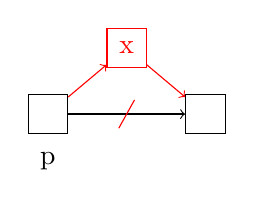
\begin{tikzpicture}[xscale = 2, yscale = 1.2]
\draw (0,0) node[draw] (p) { }; \draw (p)++(0,-0.5) node{\sm p};
\draw (p)++(1,0) node[draw] (n) { }; \draw[->] (p) -- (n);
% new node
\draw (p)++(0.5,0.7) node[draw,\new] (new) {\mbox{\scalastyle\color{\new} x}};
\draw[->, \new] (p) -- (new); \draw[->, \new] (new) -- (n);
\draw[\new] (p)++(0.45,-0.15) -- ++(0.1,0.3);
\end{tikzpicture}
%
\hfil
%
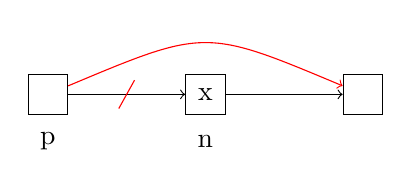
\begin{tikzpicture}[xscale = 2, yscale = 1.2]
\draw (0,0) node[draw] (p) { }; \draw (p)++(0,-0.5) node{\sm p};
\draw (p)++(1,0) node[draw] (n) {\sm x};  \draw (n)++(0,-0.5) node{\sm n};
\draw[->] (p) -- (n);
\draw (n)++(1,0) node[draw] (next) { }; \draw[->] (n) -- (next);
% updates
\draw[->, \new] (p) .. controls (1.0,0.7) .. (next);
\draw[\new] (p)++(0.45,-0.15) -- ++(0.1,0.3);
\end{tikzpicture}
\end{center}
\caption{Operations on a linked list: adding a node (left), and removing a node
  (right).}
\label{fig:linkedlist-ops}
\end{figure}

%%%%%

The |remove(x)| operation traverses the list until it finds a node~|p| such that
$\sm{p.next} = \sm{null}$ or $\sm{p.next.datum} \ge \sm{x}$.  In the case that
$\sm{p.next.datum} = \sm{x}$, it updates |p.next| to point to |n.next|.  This
is depicted in Figure~\ref{fig:linkedlist-ops} (right).

What about concurrency?  We will take the linearization points of a successful
|add| or |remove| operation to be the point at which the relevant |next| field
is updated.  First, note that when a thread~$t$ updates |p.next|, to insert or
delete a node, $t$ should have~|p| locked.  Otherwise there is an obvious race
condition: two threads could update |p.next| concurrently, and one of those
updates would be lost.  Also, $t$ should lock~|p| before reading its |next|
field, to avoid races.  Further, when deleting a node~|n|, thread~$t$ should
lock~|n| and read its |next| field first: otherwise, another thread could
update |n.next| after~$t$ has read it, and that latter update would be lost.

It is also necessary to perform locking while traversing the list, searching
for the relevant node.  If not it is possible for a thread~$t$ to find the
relevant predecessor node~|p|, but for another thread to delete~|p| before $t$
locks it.  This would mean that $t$'s updates would be lost.


%%%%%

\begin{figure}
\begin{scala}
  /** Find the first node £p£ that such that £p.next = null£ or £p.next.datum $\ge$ x£.
    * £p£ will be locked on return, and not removed from the list. */  
  private def find(x: A): Node = {
    var p = header; p.lock()
    // Invariant: all nodes £n£ before £p£ have £n.next.datum $<$ x£; £p£ is locked 
    // and in the linked list.
    while(p.next != null && p.next.datum < x){
      val n = p.next; n.lock(); p.unlock(); p = n
    }
    p
  }

  /** Does this contain £x£? */
  def contains(x: A): Boolean = {
    val p = find(x); val n = p.next; p.unlock()
    n != null && n.datum == x
  }

  /** Add £x£ to this.  Return £true£ if £x£ was not already in the set. */
  def add(x: A): Boolean = {
    val p = find(x); val n = p.next
    if(n == null || n.datum > x){ 
      p.next = new Node(x, n); p.unlock(); true 
    }
    else{ assert(n.datum == x); p.unlock(); false }
  }

  /** Remove £x£ from this.  Return £true£ if £x£ was previously in the set. */
  def remove(x: A): Boolean = {
    val p = find(x); val n = p.next
    if(n != null && n.datum == x){
      n.lock(); p.next = n.next; p.unlock(); true
    }
    else{ p.unlock(); false }
  }
\end{scala}
\caption{Operations on the linked list.}
\label{fig:LinkedListSet2}
\end{figure}

%%%%%

The |find(x)| function in Figure~\ref{fig:LinkedListSet2} performs the searching
for each of the public operations.  It returns the node~|p| before the node
where |x| might be stored, or before where |x| should be inserted.  It
guarantees that |p| is locked on return, and also that |p| has not been
deleted by another thread.  

The |find| function locks and unlocks nodes as it traverses the list.  In
particular, if the current value of~|p| has not yet reached the desired node,
it obtains the next node~|n| and locks it \emph{before} unlocking~|p| and
advancing~|p| to~|n|.  As discussed above---and as we will see below---a node
is removed from the list only when it and its predecessor are locked.  This
means that throughout the loop, |p|~references a node that has not been
removed:
% 
\begin{itemize}
\item This is certainly true initially, when the thread sets |p = header|;

\item On each iteration, when it reads |n = p.next|, it has |p| locked, so |n|
  cannot be deleted; and it locks~|n| before unlocking~|p|, so |n| still
  cannot be deleted; hence each iteration maintains this property.
\end{itemize}

\begin{instruction}
Make sure you understand the implementation of |find|.
\end{instruction}

Suppose the list contains nodes~$n_0, n_1, n_2, n_3, \ldots$, in that order.
Then the sequence of |lock| and |unlock| operations will be of the form
\[\mstyle
n_0.\sm{lock()}, n_1.\sm{lock()}, n_0.\sm{unlock()}, n_2.\sm{lock()},
n_1.\sm{unlock()}, n_3.\sm{lock()}, n_2.\sm{unlock()}, \ldots.
\]
This cannot be achieved using |mutex| blocks.  The duration of a |mutex| block
is defined syntactically by its brackets.  That means that |mutex| blocks must
follow normal bracketing rules: two |mutex| blocks should either be one inside
the other, or completely disjoint.  That is not the case with the periods
during which the thread has different nodes locked above.

This style of locking---where a thread repeatedly holds the lock on a
thread~|p|, and obtains the lock on the next node before unlocking~|p|---is
known as \emph{hand-over-hand} locking, by analogy with how one might haul on
a rope in a hand-over-hand way, repeatedly holding the rope with one hand, and
then grasping the rope with the other hand before releasing the first hand.

The public operations are then fairly straightforward.  Each uses |find(x)| to
find the predecessor node~|p|, and then relies on the guarantees that |find|
provides.  It is important to remember to unlock relevant nodes on every
branch. 

The |contains(x)| operation tests whether the node after~|p| exists
and holds~|x|.  The |find| operation guarantees that if |x| is anywhere in the
list, it is in |p.next|.  We can take the linearization point to be where the
operation reads |p.next|.  Note that it is not necessary to lock~|n|, because
the operation only reads |n.datum|, which is immutable. 

The |add(x)| operation tests whether |p.next| already contains~|x|, and if not
adds a new node containing~|x| after~|p|.  In the successful case, we can take
the linearization point to be the update of |p.next|, i.e.~the point at which
the node containing~|x| is added to the linked list.  In the unsuccessful case
we can take the linearization point to be where the thread finds that the
condition of the |if| statement fails: because of the properties of |find|, we
can be sure that |x| is not in the list at this point.  

The |remove(x)| operation tests whether $\sm n = \sm{p.next}$ contains~|x|.
If so, it locks~|n| so as to prevent any other thread changing |n.next|, as
described earlier.  It then updates |p.next| to |n.next|.  We can take the
linearization point to be this update, i.e.~the point at which |n| is removed
from the linked list.  In the unsuccessful case, we can take the linearization
point to be where the thread finds that the condition of the |if| statement
fails: the properties of |find| guarantee that |x| is not in the list at this
point.  There is no need to unlock~|n| since no thread will try to access it
subsequently. 

\begin{instruction}
Make sure you understand the implementations of these operations, and why they
are correct.
\end{instruction}

 % linked list example

%%%%%%%%%%%%%%%%%%%%%%%%%%%%%%%%%%%%%%%%%%%%%%%%%%%%%%%

\section{Summary}

In this chapter we have studied locks.  The idea is simple: a thread may
acquire a lock, and then release it: the acquiring blocks while another thread
holds the lock, so at most one lock can be held at a time.  

Locks provide a convenient way to provide mutual exclusion, so as to protect
shared state.  Each thread may access the shared state only when holding the
lock.  In particular, this provides an easy way to implement many concurrent
objects, such as total concurrent datatypes.

Locks in SCL are reentrant: a thread that holds a lock may acquire it again;
it must release the lock as many times as it acquired ut before another thread
can acquire it.  Locks provide suitable memory guarantees: if a thread writes
a value to a variable when holding a lock, that value will be available to
a subsequent thread that holds the lock.

In many cases, it is enough to protect a concurrent object using a single
thread.  However, if that object acts as a bottleneck, it can be appropriate
to use a finer granularity of locking.  In particular, sharding provides a
straightforward approach to implementing concurrent datatypes such as sets and
mappings. 



%% Other languages use similar mechanisms.  For example,
%% C++ |mutex|s act in the same way.




%%%%%%%%%%%%%%%%%%%%%%%%%%%%%%%%%%%%%%%%%%%%%%%%%%%%%%%

\exercises

\begin{questionS}
\label{ex:summer-monitor}
Give an implementation of the |Collector| trait from
Figure~\ref{fig:BoT-interfaces} using a lock.
\end{questionS}

%%%%%

\begin{answerS}
This is straightforward: the implementation encapsulates a lock, and each
operation uses the lock to provide mutual exclusion.
% 
\begin{scala}
class CollectorLock extends Collector{
  /** The sum so far. */
  private var sum = 0.0

  /** Lock protecting £sum£. */
  private val lock = new Lock

  /** Add £x£ to the result. */
  def add(x: Double) = lock.mutex{ sum += x }

  /** Get the result. */
  def get = lock.mutex{ sum }
}
\end{scala}
\end{answerS}
 % Summer for trapezium rule

\begin{questionS}
\label{ex:sharded-map}
Implement a sharded map.  (You might use code from Figure~\ref{fig:Sharding}
in your code.)  Your implementation should extend the trait |Map| in
Figure~\ref{fig:Map-trait}.  The |get(k)| operation should return a result of
type |Option[V]|: either |Some(v)| if |k| is associated with~|v|, or |None| if
|k| is not associated with any value.  Likewise, the |put| and |remove|
operations should return a result of type |Option[V]| corresponding to the
previous association of the key.  (These operations correspond to operations
from the API trait |scala.collection.mutable.Map|.)

%%%%%

\begin{figure}
\begin{scala}
trait Map[K,V]{
  /** Optionally get the value associated with £k£. */
  def get(k: K): Option[V] 

  /** Add the association £k $\rightarrow$ v£.  Optionally return the value previously
    * associated with £k£. */
  def put(k: K, v: V): Option[V] 

  /** Remove any association for £k£.  Optionally return the value previously
    * associated with £k£. */
  def remove(k: K): Option[V] 
}
\end{scala}
\caption{A trait representing mappings from {\scalashape K} to {\scalashape
    V}.}
\label{fig:Map-trait}
\end{figure}

%%%%%

Test your implementation using the linearizability testing framework.
\end{questionS}

%%%%%%%%%%

\begin{answerS}
My code is below.  This is a straightforward adaptation of the
implementation of a shared set from the body of the chapter. 

%%%%%
 
\begin{scala}
/** A sharded map from £K£ to £V£, using £shards£ shards. */
class ShardedMap[K,V](shards: Int) extends Map[K,V]{
  require(shards > 1)

  /** The amount to shift hash codes to obtain the index of the relevant
    * shard. */
  private val shift = 32-logShards(shards)

  /** The shard in which £k£ is stored. */ 
  private def shardFor(k: K) = improve(k.hashCode) >>> shift

  /** The shards.  This £ShardedMap£ object represents the union of maps. */ 
  private val maps = 
    Array.fill(shards)(new scala.collection.mutable.HashMap[K, V])

  /** Locks to protect sets: £locks(i)£ protects £sets(i)£. */
  private val locks = Array.fill(shards)(new Lock)

  /** Add the association £k $\rightarrow$ v£.  Optionally return the value previously
    * associated with £k£. */
  def put(k: K, v: V): Option[V] = {
    val s = shardFor(k); locks(s).mutex{ maps(s).put(k, v) }
  }

  /** Optionally get the value associated with £k£. */
  def get(k: K): Option[V] = {
    val s = shardFor(k); locks(s).mutex{ maps(s).get(k) }
  }

  /** Remove any association for £k£.  Optionally return the value previously
    * associated with £k£. */
  def remove(k: K): Option[V] = {
    val s = shardFor(k); locks(s).mutex{ maps(s).remove(k) }
  }
}
\end{scala}

Testing using the linearizability framework is also straightforward.  We can
use an immutable |HashMap| as the sequential specification object, with
sequential operations as follows:
%
\begin{scala}
  type SeqMap = scala.collection.immutable.HashMap[Int,Int]

  def seqPut(k: Int, v: Int)(s: SeqMap): (Option[Int], SeqMap) = 
    (s.get(k), s + (k -> v))

  def seqGet(k: Int)(s: SeqMap): (Option[Int], SeqMap) = 
    (s.get(k), s)

  def seqRemove(k: Int)(s: SeqMap): (Option[Int], SeqMap) = 
    (s.get(k), s - k)
\end{scala}

Each worker should repeatedly perform random operations, using keys from a
fairly small range, say $\interval{0}{200}$.  Other aspects of the testing are
standard. 
\end{answerS}
 %  Sharded map.

\begin{question}
Implement a map, with the same interface as in Exercise~\ref{ex:sharded-map},
using a linked list with fine-grained locking.  Give you implementation the
following signature
\begin{scala}
class LinkedListMap[K,V] (implicit ord: K => Ordered[K]) extends Map[K,V]
\end{scala}
%
The linked list should be ordered by the keys (type~|K|).

Test your implementation using the linearizability testing framework. 
\end{question}

%%%%%

\begin{answerI}
My code is below.  The definitions of nodes and the |find| function are
straightforward adaptations of those for a sharded set.  Each of the main
operations requires a little thought.  The |key| field of |n = p.next| is
immutable, so it is not necessary to lock~|n| to access it.  However, it is
necessary to lock~|n| to obtain its |value| field.  Of course, we need to
remember to unlock relevant nodes in each branch. 

%%%%%

\begin{scala}
/** An implementation of a £Map£, using a linked list. */
class LinkedListMap[K,V] (implicit ord: K => Ordered[K]) extends Map[K,V]{
  /** Nodes from which the linked list is constructed.
    * Any access to the £next£ field must be done while holding the lock on this 
    * node.  */
  private class Node(val key: K, var value: V, var next: Node){
    /** A lock used to protect the £next£ field. */
    private val l = new Lock

    /** Lock this node. */
    def lock() = l.acquire()

    /** Unlock this node. */
    def unlock() = l.release()
  }

  /** A dummy header node. */
  private val header = new Node(null.asInstanceOf[K], null.asInstanceOf[V], null)

  /* Datatype invariant: the nodes from £header.next£ onwards are in strictly
   * increasing order of £key£ fields. */ 

  /** Find the first node £p£ that such that £p.next = null£ or £p.next.key $\ge$ k£.
    * £p£ will be locked on return. */  
  private def find(k: K): Node = {
    var p = header; p.lock()
    // Invariant: all nodes £n£ before £p£ have £n.next.key $<$ k£; £p£ is locked.
    while(p.next != null && p.next.key < k){
      val n = p.next; n.lock(); p.unlock(); p = n
    }
    p
  }

  /** Optionally get the value associated with £k£. */
  def get(k: K): Option[V] = {
    val p = find(k); val n = p.next
    if(n != null && n.key == k){ 
      n.lock(); p.unlock(); val res = n.value; n.unlock(); Some(res) 
    }
    else{ p.unlock(); None }
  }

  /** Add the association £k $\rightarrow$ v£.  Optionally return the value previously
    * associated with £k£. */
  def put(k: K, v: V): Option[V] = {
    val p = find(k); val n = p.next
    if(n != null && n.key == k){
      n.lock(); p.unlock(); val res = n.value; n.value = v; n.unlock(); Some(res)
    }
    else{ p.next = new Node(k, v, n); p.unlock(); None }
  }

  /** Remove any association for £k£.  Optionally return the value previously
    * associated with £k£. */
  def remove(k: K): Option[V] = {
    val p = find(k); val n = p.next
    if(n != null && n.key == k){
      n.lock(); p.next = n.next; p.unlock(); Some(n.value)
    }
    else{ p.unlock(); None }
  }
}
\end{scala}

Testing can be done as in Exercise~\ref{ex:sharded-map}.
\end{answerI}
 % map based on linked list

\begin{question}
An \emph{iterator} is an object that supports iteration over a sequence of
values, for example the values in a collection.  In a sequential setting, an
iterator has signature as follows.
%
\begin{scala}
trait Iterator[A]{
  /** Does the sequence have a next value, i.e. is it non-empty? */
  def hasNext: Boolean

  /** Remove and return the next element from the sequence.
    * Precondition: the sequence is non-empty. */
  def next(): A
}
\end{scala}
%
The normal way in which an iterator |iter| is used in a sequential setting is
as follows:
%
\begin{scala}
while(iter.hasNext){
  val x = iter.next(); ... // Do something with £x£.
}
\end{scala}
%
This question explores how we can iterate over a sequence in a concurrent
setting.

%%%%%

\begin{enumerate}
\item
Why would the above signature and usage be inappropriate in a concurrent
setting, where several threads are using the same iterator?
%
Suggest a different signature for an iterator that is used concurrently, by
defining a trait:
%
\begin{scala}
trait ConcurrentIterator[A]{ ... }
\end{scala}
Make clear the intended meaning of any operation of this trait.
%
Give code showing how each thread would use a concurrent iterator with your
suggested signature, corresponding to the above code fragment for a sequential
iterator.  Note that the precise order in which the elements of the sequence
are handled does not matter, providing each is dealt with precisely once.

%%%%%

\item
Give a definition of a class
%
\begin{scala}
class ArrayIterator[A](a: Array[A]) extends ConcurrentIterator[A]{ ... }
\end{scala}
%
that allows iteration over the elements of the array~|a|.  The implementation
should use a |Lock| internally.

You may assume that no other thread performs and update to the underlying
array~|a| while the iteration is proceeding.  You may make similar assumptions
in the following parts. 

%%%%%

\item
The  |ArrayIterator| object is likely to act as a bottleneck.  Give an
implementation of a class
%
\begin{scala}
class ArrayBlockIterator[A](a: Array[A], blockSize: Int)
    extends ConcurrentIterator[Iterator[A]]{ ... }
\end{scala}
%
that allows each thread to obtain a sequential iterator over a block of entries
from the array of size |blockSize| (or the remainder of the array, if
fewer than |blockSize| entries are left).  Give code showing how each thread
would use such an object.  Why might this approach be better than that in the
previous part? 

%%%%%

\item
Suppose a program requires threads to collectively iterate over all values in
a sharded set.  Augment the |ShardedSet|  definition from
Section~\ref{sec:sharding} with a function
%
\begin{scala}
  def iteratorIterator: ConcurrentIterator[Iterator[A]] = ...
\end{scala}
%
Each |Iterator| produced by the |ConcurrentIterator| should be a sequential
iterator over one shard of the sharded set.  (The class
|scala.collection.mutable.HashSet| used internally in |ShardedSet| has an
operation |iterator| that produces an iterator over the |HashSet|.)

Briefly describe how threads would operate in this case.  (Full code is not
required.)  

You many assume that no other threads to attempt concurrent updates to the
sharded set while this iteration is proceeding.
\end{enumerate}
\end{question}

%%%%%%%%%%%%%%%%%%%%%%%%%%%%%%%%%%%%%%%%%%%%%%%%%%%%%%%

\begin{answerI}
\begin{enumerate}
\item
Suppose the iterator contains precisely one element, and two threads call
|hasNext|, both getting result |true|.  Then both will call |next()|.  But
they cannot both obtain the one element, so in one case the precondition will
fail.  This is a time-of-check to time-of-use error.

A possible interface is
\begin{scala}
trait ConcurrentIterator[A]{
  /** Optionally get the next element from the sequence.  
    * Return £None£ if the sequence is empty. */
  def getNext(): Option[A]
}
\end{scala}

Then each thread would do something like
\begin{scala}
var done = false
while(!done) iter.getNext() match{
  case Some(x) => ... // Do something with £x£.
  case None => done = true
}
\end{scala}

%%%%%

\item % (b)
My code is below.  The implementation uses a lock internally.
%
\begin{scala}
class ArrayIterator[A](a: Array[A]) extends ConcurrentIterator[A]{
  private val n = a.length

  /** The index of the next value to return, or £n£ if the iteration is
    * complete. */
  private var i = 0

  /** Lock to protect £i£. */
  private val lock = new Lock

  def getNext(): Option[A] = lock.mutex{
    if(i < n){ i += 1; Some(a(i-1)) } else None
  }
}
\end{scala}

%%%%%

\item
My code is below.  The concurrent iterator again uses a lock internally.
However, each |BlockIterator| that it produces will be used sequentially, so
does not need to use locking.  
%
\begin{scala}
class ArrayBlockIterator[A](a: Array[A], blockSize: Int)
    extends ConcurrentIterator[Iterator[A]]{

  /** A sequential iterator over £a[start..end)£. */
  class BlockIterator[A](a: Array[A], start: Int, end: Int) extends Iterator[A]{
    /** Index of the next element. */
    private var index = start

    def hasNext = index < end

    def next() = { require(index < end); val x = a(index); index += 1; x }
  }

  /** Index of the start of the next block. */
  private var index = 0

  /** Lock to protect £index£. */
  private val lock = new Lock

  def getNext() = lock.mutex{
    if(index < a.length){
      val start = index; index = (index+blockSize) min a.length
      Some(new BlockIterator(a, start, index))
    }
    else None
  }
}
\end{scala}
%
Given an |ArrayBlockIterator| |bIter|, a thread can do something like the
following.
%
\begin{scala}
  var done = false
  while(!done) bIter.getNext() match{
    case Some(iter) => 
      while(iter.hasNext){ 
        val x = iter.next(); ... // Do something with £x£. 
      }
    case None => done = true
  }
\end{scala}

The point is that that most of the time, each thread is operating on a
sequential object, so avoiding bottlenecks.  Also, each call to |getNext| runs
in $O(1)$ time: an approach that copies data here would be inefficient.

%%%%%

\item
My code is below.
\begin{scala}
  def iteratorIterator = new ConcurrentIterator[Iterator[A]]{
    /** The index of the next shard over which to provide an Iterator. */
    private var index = 0

    /** Lock to protect £index£. */
    private val lock = new Lock

    /** Try to get the next £Iterator£. */
    def getNext(): Option[Iterator[A]] = lock.mutex{
      if(index < shards){ index += 1; Some(sets(index-1).iterator) } else None
    }
  }
\end{scala}
%
Threads would use such an object much as in the previous part.
\end{enumerate}
\end{answerI}
 % concurrent iterators.

% Optimistic locking?  I think not.




